\documentclass[12pt, letterpaper]{article}
\usepackage[utf8]{inputenc}
\usepackage{graphicx}  % Required for inserting images
\usepackage{amssymb}
\usepackage{amsmath}
\usepackage{enumitem}
\usepackage{fancyhdr}
\usepackage{geometry}

\graphicspath{ {./images/} }
\geometry{margin = 1in}
\renewcommand{\arraystretch}{1.5}
\linespread{2}

% Macros
\newcommand{\onespace}{\hspace*{1ex}}
\newcommand{\skipline}{\\[2\baselineskip]}
\newcommand{\tab}{\hspace*{4ex}}

\title{ECS 132 Term Project}
\author{\\ Ethan Wang}
\date{}
\pagestyle{fancy}
\setlength{\headheight}{41.68335pt}
\setlength\parindent{14pt}

\begin{document}

\maketitle

% Exponential Family
\newpage
\noindent
\section*{Exponential Distribution}
\normalsize
The dataset ``adult\$capital\_gain" from fairml in the FairMLCourse repo seems to follow an exponential distribution PDF's shape \\
Initial Density Estimates\\
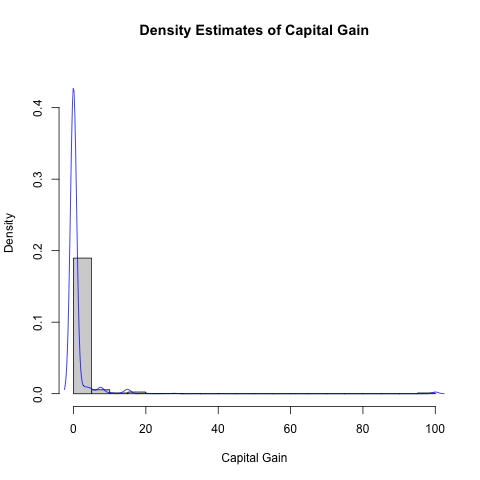
\includegraphics[scale=0.9]{capital_gain_density_estimates}
\newpage
\noindent
Using method of moments to estimate $\lambda$
\begin{flalign*}
    E(X) &= \frac{1}{\lambda}, L = \lambda\\
    \overline{A} &= \frac{1}{L}\\
    L &= \frac{\ 1\ }{\overline{A}}\\
    &\approx 0.916
\end{flalign*}
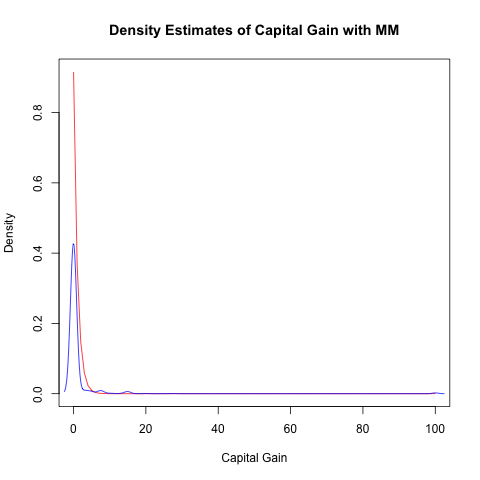
\includegraphics[scale=0.9]{capital_gain_mm}
\footnotesize
\\ \**The blue curve is the plot of density(), the red curve uses the MM estimated $\lambda$ in a plot of dexp()
\newpage
\noindent
\normalsize
Using method of maximum likelihood to estimate $\lambda$\\
Log Likelihood Expression Derivation
\begin{flalign*}
    \prod^{n}_{i = 1} {\lambda}e^{-{\lambda}X_i} &= {\lambda}^ne^{-{\lambda}\sum^{n}_{i=1}X_i}
    \\[1\baselineskip]
    \ln(\frac{\lambda^n}{e^{{\lambda}\sum^{n}_{i=1}X_i}}) &= \ln(\lambda^n) - \ln(e^{{\lambda}\sum^{n}_{i=1}X_i})\\
    &= n\ln(\lambda) - {\lambda}\sum^{n}_{i=1}X_i
    \\[1\baselineskip]
    \text{MLE estimated } \lambda &\approx 0.916
\end{flalign*}
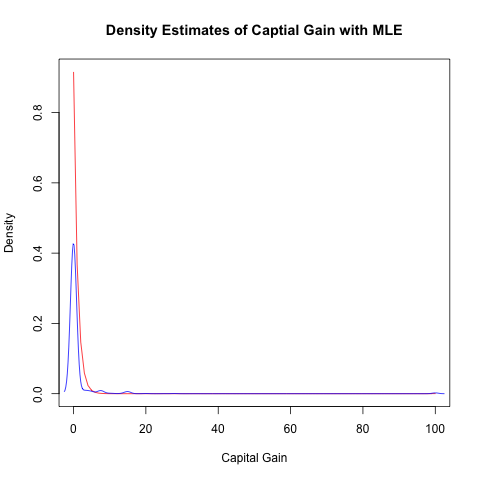
\includegraphics[scale=0.9]{capital_gain_mle}
\footnotesize
\\ \**The blue curve is the plot of density(), the red curve uses the MLE estimated $\lambda$ in a plot of dexp()
\newpage
\noindent
\normalsize
In Professor Matloff's fastStat lesson, ``MLEMM: General Methods of Estimation," both the method of 
moments estimator and the maximum likelihood estimator for the parameter $\lambda$ of an exponential 
distribution was $\frac{\ 1\ }{\overline{A}}$. However, the mle function from the stats4 
library was used to estimate $\lambda$ instead of using $\frac{\ 1\ }{\overline{A}}$ directly for the 
maximum likelihood estimator, both for consistency across our work and as an extra verification measure. 
As expected, both estimators yielded a result of about 0.916. The graph of the exponential distribution 
PDF using the estimated $\lambda$ closely follows that of the density curve of the data, which suggests 
that an exponential distribution is a suitable approximation for the population density of this dataset. An initial concern was the fact that there was a peak in the original density graph rather than a pure exponential curve and that there was a positive, nonzero density region to the left of zero. However, the exponential distribution is still believed to approximate the dataset well since there are no actual capital gain values less than zero in the dataset and a Google search revealed that the density region to the left of zero in the graph is a result of the kernel density estimation the density function does for the capital gain values equal to zero.
\\[0.5\baselineskip]
By reducing the range of the random variables to the interval zero to thirty (creating a ``new" dataset), the resulting gamma PDFs using $\lambda$ estimated by MM/MLE on the new dataset seem to fit the density graph better (see below).
\\
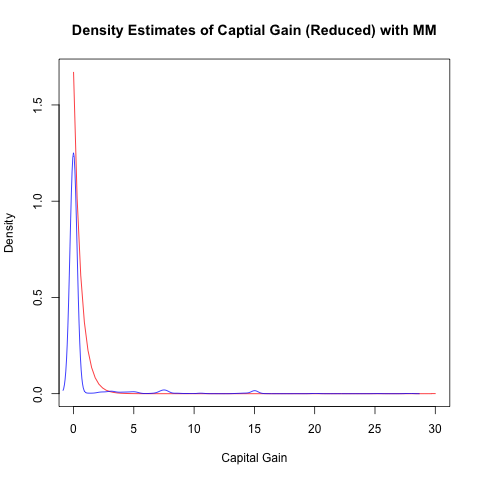
\includegraphics[scale=0.9]{capital_gain_reduced_mm}
\footnotesize
\\ \**The blue curve is the plot of density() with the reduced range, the red curve uses the new MM estimated $\lambda$ in a plot of dexp()
\\
\normalsize
However, since the nature of the data is unknown, there is no justification for cutting out the larger values from the dataset.

% Gamma Family
\newpage
\noindent
\section*{Gamma Distribution}
\normalsize
The dataset ``prgeng\$age" from qeML in the FairMLCourse repo seems to follow a gamma distribution PDF's shape \\
Initial Density Estimates\\
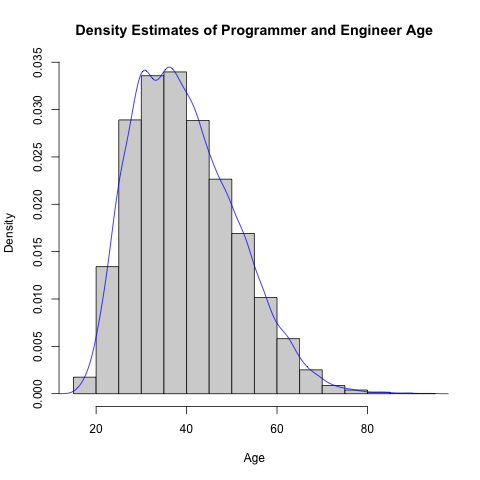
\includegraphics[scale=0.9]{prgeng_age_density_estimates}
\newpage
\noindent
Using method of moments to estimate $\lambda$ and $r$
\begin{flalign*}
    E(X) &= \frac{r}{\lambda}, L = \lambda, R = r\\
    \sigma^2 &= \frac{r}{\lambda^2}\\
    \overline{A} &= \frac{R}{L}\\
    S^2 &= \frac{R}{L^2}\\
    \\[1\baselineskip]
    R &= L\overline{A}\\
    S^2 &= \frac{L\overline{A}}{L^2}\\
    &= \frac{\overline{A}}{L}\\
    L &= \frac{\overline{A}}{S^2}\\
    &\approx 0.314\\
    R &\approx 12.421
\end{flalign*}
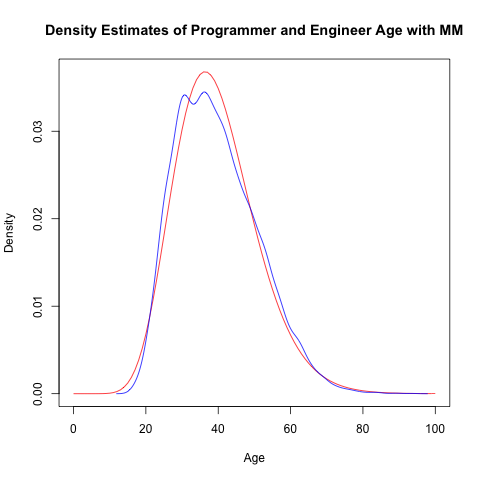
\includegraphics[scale=0.9]{prgeng_age_mm}
\footnotesize
\\ \**The blue curve is the plot of density(), the red curve uses the MM estimated {$\lambda$} and $r$ in a plot of dgamma()
\newpage
\noindent
\normalsize
Using method of maximum likelihood to estimate $\lambda$ and r\\
Log Likelihood Expression Derivation
\begin{flalign*}
    \prod^{n}_{i = 1} \frac{{\lambda}^rX_i^{r-1}}{\Gamma(r)e^{{\lambda}X_i}} &= (\frac{\lambda^r}{\Gamma(r)})^n \ast \prod^n_{i=1}X_i^{r-1} \ast \frac{1}{e^{{\lambda}\sum^n_{i=1}X_i}}
    \\[1\baselineskip]
    \ln((\frac{\lambda^r}{\Gamma(r)})^n \ast \prod^n_{i=1}X_i^{r-1} \ast \frac{1}{e^{{\lambda}\sum^n_{i=1}X_i}}) &= \ln(\lambda^{rn}) + \ln(\prod^n_{i=1}X_i^{r-1}) - \ln(e^{{\lambda}\sum^{n}_{i=1}X_i}) - \ln((\Gamma(r))^n)\\
    &= rn\ln(\lambda) + (r-1)\sum^n_{i=1}\ln(X_i) - {\lambda}\sum^{n}_{i=1}X_i - n\ln(\Gamma(r))
    \\[1\baselineskip]
    \text{MLE estimated } \lambda &\approx 0.320\\
    \text{MLE estimated } r &\approx 12.643
\end{flalign*}
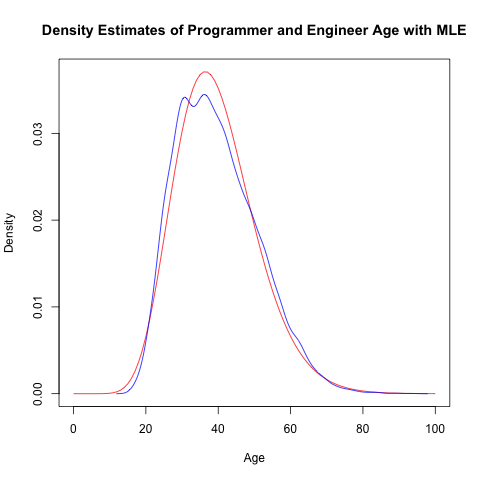
\includegraphics[scale=0.9]{prgeng_age_mle}
\footnotesize
\\ \**The blue curve is the plot of density(), the red curve uses the MLE estimated {$\lambda$} and $r$ in a plot of dgamma()
\newpage
\noindent
\normalsize
For the dataset chosen to be approximated by a gamma distribution, the estimated values for $\lambda$ and $r$ 
have little difference from one method of forming estimators to the other. The graphs of the gamma 
distribution PDF using the estimated $\lambda$ and $r$ parameters for each estimation fit the density 
curve of the dataset well, suggesting that a gamma distribution is a suitable approximation for the 
population density of this dataset. One concern is that the peaks of both PDFs are slightly to the right 
of the one in the original density graph. Since the difference in peak locations is pretty small, the suitability of the gamma distribution in approximating the population density of the dataset remains unchanged.
\\[0.5\baselineskip]
Another concern was the slight dip in the peak of the density graph of the dataset. While playing with the bandwidth parameter, a bandwidth value of four got rid of the dip, as depicted below.
\\
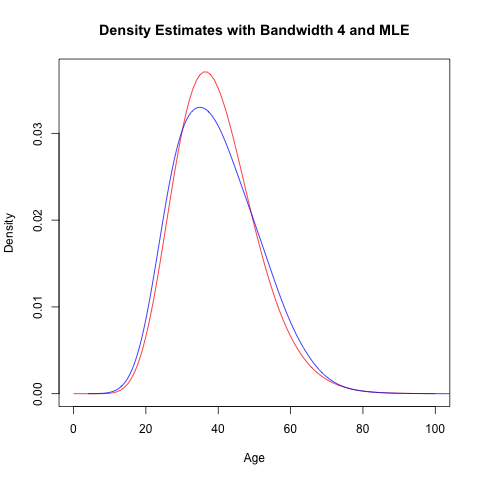
\includegraphics[scale=0.9]{prgeng_age_bandwidth_4}
\footnotesize
\\ \**The blue curve is the plot of density() with bw=4, the red curve is the same MLE graph as above \\
\normalsize
However, a bandwidth of four felt like too much smoothing since it is very likely that this small dip is a result of sample variability. The reasoning behind this is one, the dip is small enough so that it does not create two peaks, and two, this dataset involves the ages of programmers and engineers, and it seems unlikely that there would be a sudden downward trend in the number of programmers and engineers around the age of 35. This bandwidth setting also makes the MLE and MM graphs less fitting.


% Contribution Section
\newpage
\begin{center}
    \section*{Team Member Contributions}
\end{center}

\normalsize
Ethan Wang
\begin{itemize}[leftmargin=50pt]
  \item Exponential and gamma distributions (data and analysis)
  \item R code in exp\_and\_gamma.R
\end{itemize}


\end{document}

